\chapter{Initial Implementation} \label{chap:initial_implementation}

\section{Data Preprocessing}

In order to begin analysing neuromorphic data, it was pre-processed it into a form that a NN can take as input. One such method of doing so was to segment the events into groups based on their timestamp. \autoref{fig:nmnist_spikes_to_intensity_map} shows a visualisation of intensity maps created from the NMNIST\cite{NMNIST} dataset. The set of all events was split into eight segments, where each segment included events within a range of $ 1 \times 10^6 $ ms (i.e., $ 0 \rightarrow 1 $, $ 1 \rightarrow 2 $, ..., $ 7 \rightarrow 8 $). This way the data representation shifted to somewhat get back to a set of frames that mimicked the video output usually seen from everyday cameras. \textbf{(a)} shows the segmented events visualised in three dimensions (x\_location, y\_location and timestamp). In \textbf{(b)} these events were projected onto the two dimensional plane (of x\_location and y\_location), then the plots for on events and off events are shown separately. Finally in \textbf{(c)} an intensity map was created from the projected events. Each pixel in the intensity map grid was initialised to 0, and for every on event 1 was added to the cell, and for every off event 1 was subtracted from the cell. It was clear that the resulting output greatly resembled the MNIST\cite{MNIST} sample recorded by the ATIS camera (As shown in \autoref{fig:nmnist_spikes_visualisation} in \Cref{sec:existing_datasets}).

\begin{figure}[htb]%
    \centering
    \subfloat[\centering]{{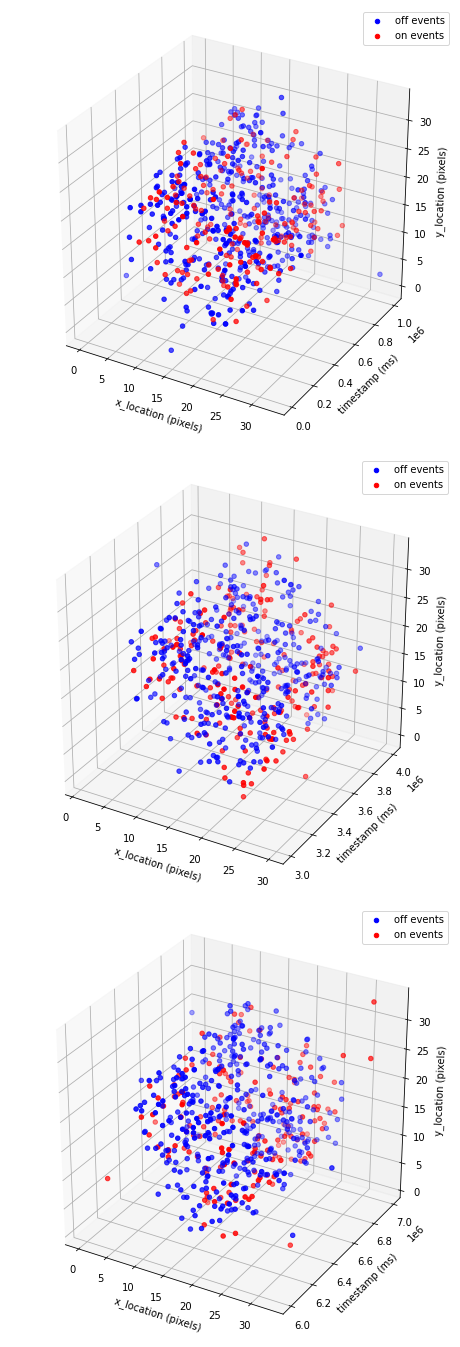
\includegraphics[width=0.25\textwidth, height=0.7\textwidth]{background/images/nmnist_spikes_visualisation_segmented.png}}}%
    \qquad
    \subfloat[\centering]{{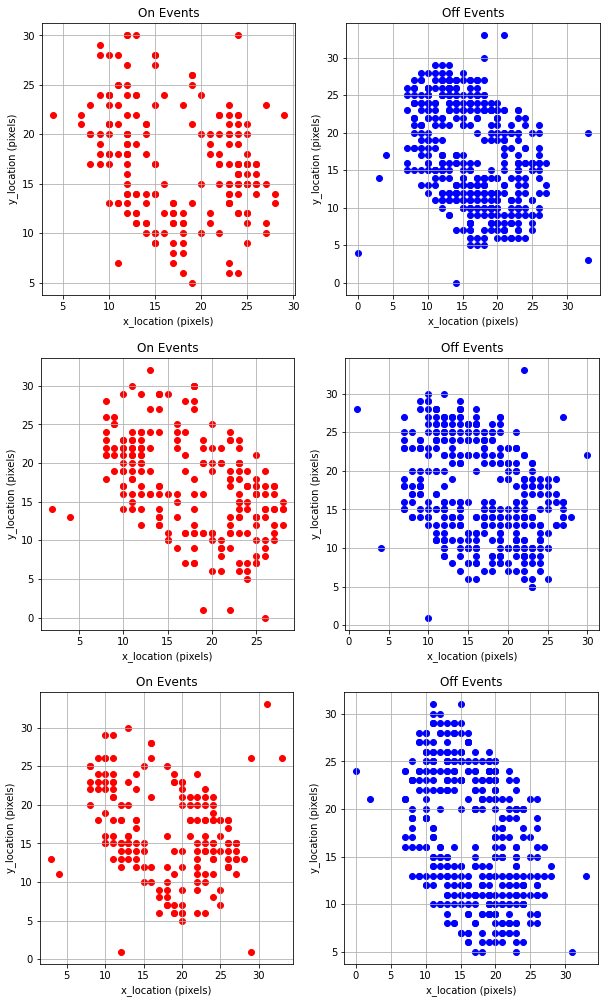
\includegraphics[width=0.4\textwidth, height=0.7\textwidth]{background/images/nmnist_events_segmented.png}}}%
    \qquad
    \subfloat[\centering]{{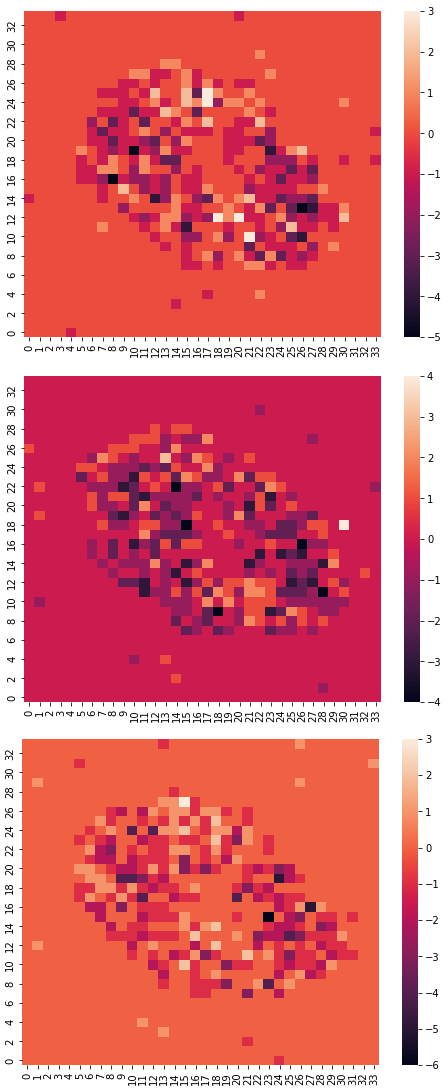
\includegraphics[width=0.25\textwidth, height=0.7\textwidth]{background/images/nmnist_events_heatmap_segmented.png}}}%
    \caption{A visualisation of intensity maps created by segmenting events into bins of size $ 1 \times 10^6 $ ms.}%
    \label{fig:nmnist_spikes_to_intensity_map}%
\end{figure}

Once a set of projections was made for each sample from the NMNIST dataset, it could be fed into a neural network in parallel. Ths could be done by simply flattening each intensity map and feeding all the cell values to a fully-connected dense layer in parallel, or the maps could be fed in as images to a convolutional layer. For the convolutional layer method a 3D tensor could be generated by stacking each of the intensity maps against each other and feeding them all directly into the first layer of the NN.

\color{red} PLEASE NOTE THAT THIS SECTION IS IN PROGRESS AND MORE WILL BE ADDED AS IT IS IMPLEMENTED \color{black}